
\section{Reinforcement Learning}
\label{section:Reinforcement-Learning}
Reinforcement learning is a machine learning technique where a learner interacts with an environment with the objective of finding which of the actions it can take will maximize the cumulative reward or \textit{return} it will receive in the long run\cite{Sutton:1998}. The learner or decision-maker is known as the \textit{agent} and everything with which the agent interacts is the \textit{environment}. How the agent behaves is defined by the \textit{policy} normally referred to as $\pi$. The policy that the agent follows specifies which \textit{actions}, $a$, the agent takes depending on the situation of the environment and, as the learning process goes on, the policy tends to improve if the problem is well formulated.  A policy can be as simple as a deterministic lookup table where for each situation the table provides an action. On the other hand, more complex stochastic policies provide a probability for each action that can be taken in each situation.

The different situations of the environment in which the agent may find itself, are the \textit{states}. A state, $s$, is a sufficient summary of what is going on in the environment and when it is possible to access all this sufficient information, the environment is said to be \textit{fully observable}. At every time step, the agent perceives an \textit{observation} that is a consequence of the state of the environment at that moment. Sometimes, just from the available observation, it is not possible to extract the state underneath and then, the environment is said to be \textit{partially observable}. The goal of the agent is to select those actions that will maximize the expected discounted return $G_t$ after $k$ time steps, see equation \ref{eq:expected-discounted-return}.
\begin{equation}
G_t = R_{t+1} + \gamma R_{t+2} + \gamma^2 R_{t+3} +... = \sum_{k=0}^{\infty} \gamma ^k R_{t+k+1}
\label{eq:expected-discounted-return}
\end{equation}

In previous equation \ref{eq:expected-discounted-return}, $\gamma$ is the \textit{discount rate}, a parameter in the range $0 \leq \gamma \leq 1$ that represents the value that future rewards have at the current time step $t$. A $\gamma$ closer to $0$ indicates that the agent favour immediate rewards whereas a $\gamma$ closer to $1$ shows an agent that strongly takes into account future rewards. At each time step $t$, the environment sends a \textit{reward signal} to the agent that indicates how well the agent is performing in the \textit{immediate} sense. On the other hand, the \textit{value} of a state indicates how desirable a state is in the \textit{long run}. In other words, the value of a state $s$, $v_\pi \left(s\right) $, is the expected discounted return $G_t$ that an agent will receive over the future if it starts interacting at that state $s$ and continues following its policy $\pi$. This is captured by the \textit{value function} shown in equation \ref{eq:value-function}:






\begin{equation}
v_\pi \left(s\right) = E_\pi \left[G_{t}\mid S_{t}=s\right]
\label{eq:value-function}
\end{equation}



Similarly, the \textit{action-value function} or \textit{Q-function}, denoted as $q_\pi$ and shown in equation \ref{eq:q-function}, tells us how good it is for the agent to take an action at a given state while following a policy $\pi$. In other words, it gives us the \textit{value of an action} under $\pi$.

\begin{equation}
q_\pi \left( s,a \right) = E_\pi \left[ G_{t}\mid S_{t}=s,A_{t}=a \right] 
\label{eq:q-function}
\end{equation}


The output of the Q-function for any given state-action pair is called the \textit{Q-value}. 

When a reinforcement learning agent starts learning in an unknown environment it has to \textit{explore} new states to discover where the best rewards are. At the same time, it has to \textit{exploit} what it already knows to choose the best actions. This is known as the \textit{exploration-exploitation }dilemma and it is a key challenge in reinforcement learning \cite{Sutton:1998}.


\subsection{Markov Decision Process (MDP)}

Reinforcement learning makes use of Markov decision processes (MDP) as a framework for sequential decision-making problems. This framework is a simple way of representing the interaction between the agent and the environment in terms of states, actions and rewards \cite{Sutton:1998}. MDPs satisfy the \textit{Markov property} that says that for a sequence of states $s_0, s_1, ..., s_t$, at any time $t$, the next state $s_{t+1}$ only depends on the current state $s_t$ \cite{Osa:2018}.

An MDP is defined by a tuple $(\mathcal{S}, \mathcal{A}, \mathcal{T}, \mathcal{R})$ where $\mathcal{S}$ is the set of states, $\mathcal{A}$ is the set of actions, $\mathcal{T}(s, a, s')$ is the \textit{transition function} and $\mathcal{R}(s, a)$ is the \textit{reward function}.

\begin{figure}[H]
    \centering
    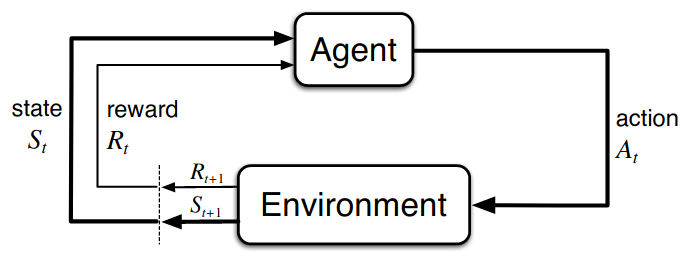
\includegraphics[width=.7\textwidth]{Figures/reinforcement_learning.png}
    \caption{Reinforcement Learning}
    \label{fig:reinforcement_learning}
\end{figure}

Figure \ref{fig:reinforcement_learning} shows the interaction between an agent and the environment in an MPD. At time step $t$, the agent finds itself at state $s_t$ and performs an action $a_t$ on the environment. Then, the environment evolves to the next state $s_{t+1}$ where the agent receives the reward $r_{t+1}$. As the learning process continues, the agent and the environment produce a sequence or \textit{trajectory $\tau$} of states, actions and rewards:


\begin{equation}
\tau = s_0, a_0, r_1,s_1, a_1, r_2,s_2, a_2, r_3, ...
\label{eq:value-function}
\end{equation}

\subsection{On-policy and off-policy Reinforcement Learning}
\label{section:on and off-policy Reinforcement Learning}
One of the objectives of this literature review is to establish a clear definition of the concepts on-policy and off-policy in the field of imitation learning. Before that, in this section we will explain the meaning of these terms in reinforcement learning, a field where they are widely used and well known. To the best of our knowledge, the first mention of the terms on-policy and off-policy in reinforcement learning is found in the book \textit{Introduction to Reinforcement Learning} by \cite{Sutton:1998}.

According to Sutton and Barto, on-policy methods use a single policy, the same policy that is evaluated or improved is the one used to generate behaviour. On the other hand, off-policy methods use two policies: They evaluate or improve a policy, the target policy, while using a different policy to generate the data, the behaviour policy. In this case, we say that learning is from data \quotes{off} the target policy, and the overall process is termed off-policy learning. \cite{Sutton:1998}. These definitions are the most accepted and used in reinforcement learning and therefore we will use them as reference further in this review. To better understand the terms, we are going to briefly explore two popular RL algorithms, Q-Learning and SARSA to understand what makes the former off-policy and the later on-policy.

\subsubsection*{Sarsa and Q-learning}
SARSA and Q-learning are Temporal Difference (TD) algorithms that update the knowledge of the agent at every time step by bootstrapping which means that the update is partly based on other learned estimates, without waiting to know the final outcome \cite{Sutton:1998}. Equation \ref{eq:TD} shows the general update rule of these TD methods \cite{TD:equation:2019}, here the \textit{step size} is equivalent to the learning rate.


\begin{equation}
\text{New estimate } \leftarrow \text{ Old estimate }+ \text{ Step size }* \left[\text{ Target - Old estimate} \right]
\label{eq:TD}
\end{equation}

Q-Learning was first introduced by \cite{Watkins:1989} and it is considered an off-policy method because if follows a behaviour policy $\beta$ while evaluating another policy $\pi$. Equation \ref{eq:Q-learning} shows the update rule for this method where $s_t$ and $a_t$ are the state and action at time step $t$, $R$ is the reward obtained for taking $a_t$ at state $s_t$, $\alpha$ is the step size or learning rate and $\gamma$ is  the discount rate. The term $\max_{a} Q(s_{t+1}, a)$ represents  the best-estimated value for the next state $s_{t+1}$ and it is independent of the policy being followed.

\begin{equation}
Q^{\text{new}}(s_t, a_t)  \leftarrow Q(s_t, a_t) + \alpha \left[ R  + \gamma {\max_{a} Q(s_{t+1}, a)} - Q(s_t, a_t)\right]
\label{eq:Q-learning}
\end{equation}


SARSA algorithm was first introduced \cite{Rummery+Niranjan:1994} with the name \quotes{Modified Connectionist Q-Learning (MCQ-L)} and it was Richard Sutton who suggested, in the same publication of Rummery and Niranjan, the name SARSA, as you need to know State-Action-Reward-State-Action before performing an update.  Unlike Q-learning, the policy that SARSA evaluates is the same with which it generates samples. Equation \ref{eq:SARSA} shows its update rule.

\begin{equation}
Q^{\text{new}}(s_t, a_t)  \leftarrow Q(s_t, a_t) + \alpha \left[R+ \gamma  Q(s_{t+1}, a_{t+1}) - Q(s_t, a_t)\right]
\label{eq:SARSA}
\end{equation}
When comparing both updating rules in equations \ref{eq:Q-learning} and \ref{eq:SARSA}, we can see that in Q-learning the agent learns the optimal policy by using a greedy policy when updating the Q-value (see the \textit{max} in equation \ref{eq:Q-learning}). This is what makes Q-learning off-policy, the fact that it can use a policy for generating behaviour different from the greedy policy with which it updates the Q-values. This is key to understand why Q-learning can make use of the experience replay technique as we will see in section \ref{sec:experience-replay}.



\subsection{Online and Offline} Reinforcement learning algorithms can also be classified according to how data is collected. Traditional RL algorithms are active or online frameworks \cite{youtube_offline_RL}, where an agent iteratively interacts in its environment collecting experience and using it to update its policy. Online RL algorithms can be on-policy if  they use data exclusively collected by the current agent, or off-policy, see table \ref{tab:RL-classification}; off-policy RL algorithms are able to use previous data but the agent continues interacting with the environment collecting more data that is added to a buffer and then uses the data from the buffer to improve its policy. This online approach works well in very specific and  simulated environments however, for real-world settings, online learning is impractical because the agent still needs to collect a diverse and huge data set at each iteration. 

Offline reinforcement learning, see table \ref{tab:RL-classification}, also called batch RL, data-driven RL or fully off-policy RL,  addresses the aforementioned problem. The key idea is that a large and diverse dataset is previously collected by some behaviour policy and added into a buffer. Then using only that data, the agent has to learn the best possible policy without further interacting with the environment. With this offline framework, it is possible to apply RL to real-world domains like robotics where the agent, the robot, could easily get damaged while collecting data iteratively in an online manner. The downside of offline learning resides in collecting a suitable dataset for training which for many real-world applications, data can be very expensive to acquire \cite{collecting_data_for_offline_learning}.





\begin{table}[]
\begin{tabular}{c|c|l|l|l|}
\cline{2-5}
\textbf{} &
  \multicolumn{2}{p{5cm}|}{\textbf{Only use data collected by current agent}} &
  \multicolumn{2}{c|}{\textbf{Use data collected by other agents}} \\ \hline
\multicolumn{1}{|p{3cm}|}{\textbf{Data collection using current agent}} &

  \multicolumn{2}{l|}{\begin{tabular}[c]{@{}l@{}}
  
Online, on-policy RL \\

  \raisebox{-\totalheight}{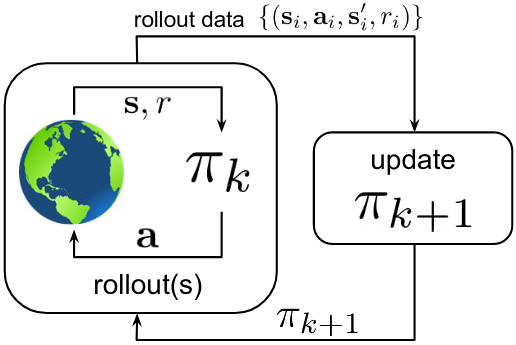
\includegraphics[width=5cm]{Figures/on-policy.png}}
  \vspace{5mm} 
  
  \end{tabular}} &
  
  \multicolumn{2}{l|}{\begin{tabular}[c]{@{}l@{}}
  
Online, off-policy RL \\

  \raisebox{-\totalheight}{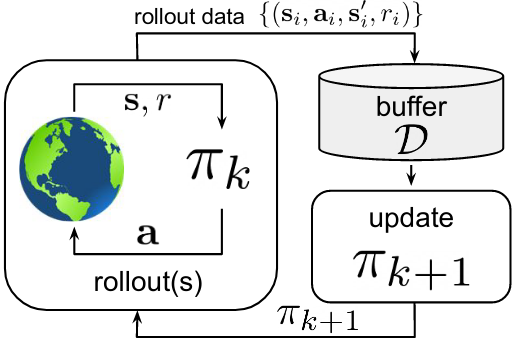
\includegraphics[width=5cm]{Figures/off-policy.png}}
  \vspace{5mm} 
  
  \end{tabular}} \\ \hline
  
\multicolumn{1}{|p{3cm}|}{\textbf{Fixed dataset (no additional data collection)}} &
  \multicolumn{2}{c|}
  {-} 
  &
  \multicolumn{2}{l|}{\begin{tabular}[c]{@{}l@{}}
  
  Offline (fully off-policy) RL \\
  
  \raisebox{-\totalheight}{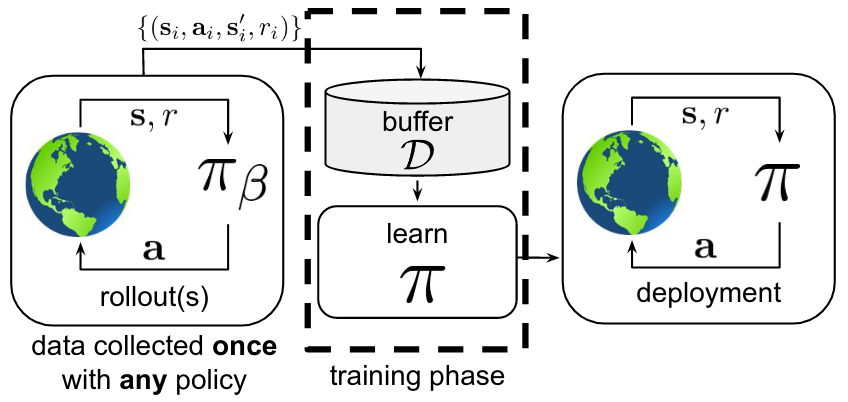
\includegraphics[width=7cm]{Figures/offline.png}}
  
  \end{tabular}} \\ \hline
\end{tabular}
\caption{Classification of RL algorithms, \cite{Google_offline_RL}, \cite{youtube_offline_RL}
and \cite{Offline-RL-Levine:2020}.}
\label{tab:RL-classification}
\end{table}











\subsection{Experience Replay}
\label{sec:experience-replay}

Experience Replay is a replay memory technique in which the transitions, $<s_t, a_t, r_{t+1}, s_{t+1}>$, gathered by an agent at every time step $t$ are stored into a memory or \textit{replay buffer}. The idea of experience replay is to randomly sample mini-batches of experience from the buffer to update the policy. 



% Three benefits are obtained with this technique: ER is an efficient manner of taking advantage of the experience that has been already collected and use it to learn multiple times \cite{Experience-Replay-zhang:2018}. On the other hand is a way to train the policy with  uncorrelated data  which makes the Neural Network  more robust against locally overfitting to the most recent trajectories, also known as a forgetting phenomenon. 

Experience replay provides several benefits. First, it is an efficient manner of taking advantage of the experience that has been already collected and use it to learn multiple times \cite{Experience-Replay-zhang:2018}. This is particularly important in the case of neural networks because it increases their stability helping to preserve old knowledge and thus reducing catastrophic forgetting \cite{Experience_replay_stability:2019}.
Furthermore, experience replay provides uncorrelated data to train the neural network which helps it to generalize and to minimize overfitting to the most recent trajectories. \cite{Machine_learning_finance:2019}.

 

To be able to use this experience replay technique, it is necessary to have an off-policy algorithm. Off-policy RL methods continue estimating the optimal Q-value, $Q^*$, even if the policy that they follow changes from $\pi_1$ to $\pi_2$. However, an on-policy method following a policy $\pi_1$ will yield a Q-value $Q_{\pi_1}$ and if the policy changes to $\pi_2$, it will yield $Q_{\pi_2}$; the optimal Q-value in this last situation will not be guaranteed. It is important to remark that even if the experiences were collected with a single policy $\pi$, because the policy evolves over time, the same policy at time step t, $\pi_t$, is not equal to that same policy in a later time step, $\pi_N$; they are considered experiences gathered by \textit{different policies} and therefore only off-policy methods are applicable.













\section{Imitation Learning}
\label{section:Imitation-Learning}

Imitation learning is a problem in machine learning where an agent learns a task leveraging the knowledge of a teacher which can be a human or a more experienced agent \cite{Imitation-Learning-definition-torabi:2019}. Imitation learning is more useful with respect to reinforcement learning when it is easier for a teacher to demonstrate or provide feedback in order for the agent to learn rather than to specify a reward function that would lead to the desired behaviour. The simplest imitation learning algorithm is called behavioural cloning where a teacher provides some initial demonstrations and the agent tries to learn a policy via supervised learning.


\subsection{Interactive Imitation Learning}
\label{sec:Interactive-Imitation-Learning}

Interactive imitation learning is a branch of imitation learning \cite{lazydagger:2021}, where the teacher interacts with the agent \textit{during} its training providing feedback to improve its behaviour, see figure \ref{fig:interactive_imitation_learning}. Some authors \cite{Osa:2018} consider these interactive techniques as a special part of behavioural cloning but to make a more clear distinction it is preferable to consider them as a branch of IL.



\begin{figure}[H]
    \centering
    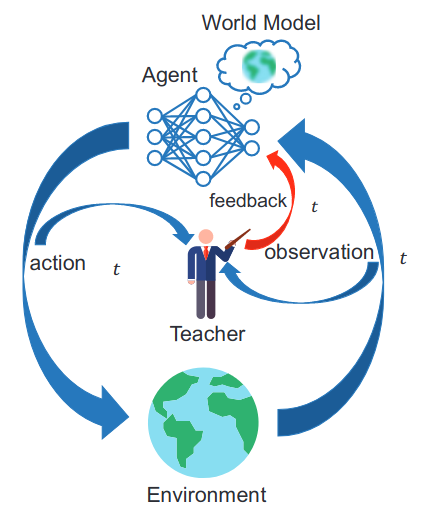
\includegraphics[width=.4\textwidth]{Figures/interactive_imitation_learning.png}
    \caption{Interactive Imitation Learning \cite{D-COACH-Dattari-Celemin-Ruiz-del-Solar-Kober:2018}}
    \label{fig:interactive_imitation_learning}
\end{figure}

 The nature of the feedback varies between frameworks: Feedback in the form of evaluations (e.g., the TAMER framework \cite{TAMER-Knox-Stone:2009}) inform the agent how good or bad was the action taken. This kind of evaluative feedback is easier to implement than to define a reward function and allows a faster convergence than pure autonomous learning. 
However, the informativeness of this kind of evaluative feedback is still limited \cite{types-feedback-najar:2020}, and one way to improve it is to use corrections. Feedback as relative corrections \cite{Relative-corrections-Celemin:2019} gives name to corrective imitation learning, a branch of IIL. Corrective feedback improves the informativeness of evaluative feedback, by allowing the teacher to inform the agent whether the value of a taken action should be increased or decreased [Celemin and Ruiz-Del-Solar, 2019]. This requires less exploration compared to evaluative feedback \cite{types-feedback-najar:2020}. Section \ref{sec:Corrective-Imitation-Learning} provides more details about corrective imitation learning.




\subsection{On-policy and off-policy Imitation Learning}
\label{section:on and off-policy Imitation Learning}

Section \ref{section:on and off-policy Reinforcement Learning} explained the meaning of the terms on-policy and off-policy in the field of reinforcement learning. When researching the literature it is clear that, for RL,  the definition provided by Sutton and Barto in 1998 is the most used. However, things are not that obvious when talking about imitation learning. According to the paper \textit{An Algorithmic Perspective on Imitation Learning} \cite{Osa:2018} the first mention to the terms on-policy and off-policy regarding imitation learning is due to \cite{DBLP:journals/corr/LaskeyLHLMFG17}. These definitions are:
\setlength{\parskip}{1em} 

\say{In Off-Policy imitation learning, an agent observes demonstrations from a supervisor and tries to recover the behaviour via supervised learning, an example of off-policy IL is behavioural cloning. On-policy imitation learning methods sample trajectories from the agent’s current distribution and update the model based on the data received. A common on-policy algorithm is DAgger.} 

\setlength{\parskip}{1em} 

Similar definitions are found in \cite{OtherLaskeydefinitions:2019} and \cite{Anotherdefinitionfromberkeley:2020}:

\say{On-policy imitation learning involves executing the current agent's policy $\pi_{\theta_i}$ in the environment allowing it to make errors and observe new states and then soliciting feedback from a supervisor on the visited states to update $\pi_{\theta_i}$. This is in contrast to off-policy imitation learning algorithms where policy learning is performed entirely on states from the supervisor's trajectory distribution.}
 
\setlength{\parskip}{1em} 

While we agree with the previous definition of on-policy IL, regarding off-policy IL, we consider that it is easier to interpret and relate its meaning to RL, simply as the opposite of on-policy IL. Therefore our reinterpretation of the definitions is:  

\begin{itemize}
  \item \textbf{On-Policy imitation learning}: \quotes{On-Policy IL methods sample trajectories using the current agent’s policy and use that data to update that same policy.}
  
  \item \textbf{Off-Policy imitation learning}: \quotes{Off-Policy IL methods sample trajectories using a policy different from the current agent’s one.}
  


\end{itemize}


In \cite{DBLP:journals/corr/LaskeyLHLMFG17}, \cite{OtherLaskeydefinitions:2019} and \cite{Osa:2018} the first example of on-policy imitation learning given is DAgger (Dataset  Aggregation) \cite{DAgger-Ross:2011}; however, according to their own definitions we consider important to make a clarification regarding this classification. Algorithm \ref{al:DAgger-simplest} shows DAgger's \textit{simplest form}. For the first iteration, DAgger uses the expert’s policy $\pi^*$ (line 2), to collect a dataset of trajectories $D$ and then, trains a policy  $\hat{\pi}_2$ that best mimics the expert on those trajectories. Then at iteration $n$, it uses $\hat{\pi}_n$ to collect more trajectories and adds those trajectories to the dataset $D$. The next policy $\hat{\pi}_{n+1}$ is the policy that best mimics the expert on the whole dataset $D$. In summary, DAgger uses its \textit{current policy} to collect a dataset at each iteration and trains the next policy under the aggregate of all collected datasets \cite{DAgger-Ross:2011}.

\begin{algorithm}[H]
\caption{The simplest version of the DAgger algorithm }
\begin{algorithmic}[1]
\State \textbf{Initialize} $\mathcal{D} \leftarrow 0$ 
\State \textbf{Initialize} $\hat{\pi}_1 \leftarrow \pi^*$ 
\For {$i = 1 $  \textbf{to} $N$} 
\State Let $\pi_i = \hat{\pi}_i$
\State Sample T-step trajectories using $\pi_i$
\State Get dataset  $\mathcal{D}_i = \{(s, \pi^*(s))\}$ of visited states by $\pi_i$ and actions given by expert
\State Aggregate datasets:  $\mathcal{D} \leftarrow \mathcal{D} \cup  \mathcal{D}_i$
\State  Train classifier $\hat{\pi}_{i+1}$ on $\mathcal{D}$
\EndFor
\State Return best $\hat{\pi}_i$ on validation
\end{algorithmic}
\label{al:DAgger-simplest}
\end{algorithm}

This simple version of DAgger fits in the definition of on-policy imitation learning found in the literature because as can be seen in lines 4 and 5 of the algorithm\ref{al:DAgger-simplest}, the policy that gathers the trajectories is the current agent's policy.


However, and to better leverage the knowledge of the expert, the authors \textit{optionally} allow the algorithm to use a modified policy $\pi_i=\beta_i\pi^{∗}+ (1−\beta_i)\hat{\pi}_i$. Depending on $\beta$,  which has values within the range $[0,1]$, the expert policy $\pi^*$, is able to collect part of the next dataset by itself. If $\beta = 1$, the expert has full control when collecting the data opposite to $\beta=0$  which means that all the data is gathered by the current agent's policy. The parameter $\beta$ can be equal to $\beta_i=p^{i−1}$ representing a decaying rate over time of the usage of the expert to collect the data.


This more generic version represented in the algorithm \ref{al:DAgger-general}would not fit into the definition of on-policy imitation learning given by \cite{Osa:2018}, \cite{DBLP:journals/corr/LaskeyLHLMFG17}, \cite{OtherLaskeydefinitions:2019} and \cite{Anotherdefinitionfromberkeley:2020} due to the fact that during the first iterations, the expert's policy has more weight than the agent's policy when collecting the data.


\begin{algorithm}[H]
\caption{DAgger algorithm with stochastic mixing of the agent and the supervisor policies }
\begin{algorithmic}[1]
\State \textbf{Initialize} $\mathcal{D} \leftarrow 0$ 
\State \textbf{Initialize} $\hat{\pi}_1 \leftarrow \pi^*$ 
\For {$i = 1 $  \textbf{to} $N$} 
\State Let $\pi_i = \beta_i\pi^* + (1 -\beta_i)\hat{\pi}_i$
\State Sample T-step trajectories using $\pi_i$
\State Get dataset  $\mathcal{D}_i = \{(s, \pi^*(s))\}$ of visited states by $\pi_i$ and actions given by expert
\State Aggregate datasets:  $\mathcal{D} \leftarrow \mathcal{D} \cup  \mathcal{D}_i$
\State  Train classifier $\hat{\pi}_{i+1}$ on $\mathcal{D}$
\EndFor
\State Return best $\hat{\pi}_i$ on validation
\end{algorithmic}
\label{al:DAgger-general}
\end{algorithm}

To summarize this section, if the teacher intervenes somehow  in the gathering of the data, we consider this imitation algorithm to be off-policy.

\subsection{Imitation Learning algorithms}

In this section, we gather and briefly describe some Imitation Learning algorithms with the objective of later classify them according to the proposed definitions from the previous subsection.




\subsubsection*{Behavioural Cloning}
Behavioural cloning (BC) \cite{Behavioural-Cloning-Pomerleau:1991}, one of the oldest Imitation Learning frameworks, consists on directly learning a policy, via supervised learning, given a data set of demonstrations provided by a teacher. The main problem with BC is known as \textit{distribution mismatch} and it happens because at the moment that the learner agent deviates from the expert trajectory, it cannot recover from that failure and go back to the expert trajectory. This provokes a cascade of errors that keep growing because the agent doesn't know how to act in those states that haven't been visited by the expert \cite{Global-overview-Attia:2018}.

\subsubsection*{DART}
DART (Disturbances for Augmenting Robot Trajectories) \cite{DART-Laskey:2017} is an algorithm close to behavioural cloning \cite{Behavioural-Cloning-Pomerleau:1991}. According to its authors is an off-policy imitation learning algorithm because, after the first expert's demonstration, it does not require to query the expert anymore. This method works by injecting noise into the supervisor's policy while demonstrating the task.

\subsubsection*{SQIL}
SQIL (Soft Q Imitation Learning) \cite{SQIL-Reddy-Dragan-Levine:2019} is a variant of behavioural cloning that incentives the agent to match human demonstrations over a long horizon. SQIL uses reinforcement learning but doesn't learn a reward function, instead, when the agent matches a demonstrated action in a demonstrated state, it receives a reward of "1" and "0" for every other behaviour.

\subsubsection*{ValueDICE}
ValueDICE (Distribution Correction Estimation) \cite{ValueDICE-Kostrikov:2019}, is an off-policy imitation learning \cite{Laskey:phdthesis} that minimizes the KL-divergence between the expert distribution and the distribution induced by the agent when interacting with the environment in an off-policy manner.

%% DAGGERS!%%%%%%%%%%%%%%%%%%%

\subsubsection*{DAgger}
DAgger (Data Aggregation) \cite{DAgger-Ross:2011} is one of the most well-known imitation learning algorithms and it was explained in-depth in section \ref{section:on and off-policy Imitation Learning}. Many variants of DAgger exist and some of them are going to be commented on next.



\subsubsection*{DAgger by coaching}
DAgger by coaching \cite{DAgger-by-coaching-He-DaumeIII-Eisner:2012},  is a version of DAgger \cite{DAgger-Ross:2011} where the human teacher executes actions that are within learner’s ability. This means that when the agent is at a state far from the desired state, the teacher won't try to correct directly that difference but instead it will try to redirect the agent gradually \cite{Global-overview-Attia:2018}.


\subsubsection*{AggreVaTe}
AggreVaTe (Aggregate Values to Imitate) \cite{AggreVaTe-Ross-Bagnell:2014}, is a version of DAgger \cite{DAgger-Ross:2011}, that learns to choose actions that minimize the cost-to-go of the expert, 
\cite{Global-overview-Attia:2018}. The cost-to-go $Q$ is the cost of executing an action in a state and continue executing a policy for the next steps. The first iteration is the same as in DAgger, then for the next iterations,  at a time t, the cost-to-go $Q$ of taking an action in a state is observed and added to the initial dataset $D$ together with the action and the state.



\subsubsection*{AggreVaTeD}
AggreVaTeD \cite{AggreVaTeD-Sun:2017} is a differentiable version of the AggreVaTe algorithm introduced by \cite{AggreVaTe-Ross-Bagnell:2014} that does not perform any data aggregation. It includes two gradient update procedures: An online gradient descent and a natural gradient update similar to exponential gradient descent.

\subsubsection*{SafeDAgger}
SafeDAgger \cite{SafeDAgger-Zhang-Cho:2016}, is a version of DAgger \cite{DAgger-Ross:2011}, that aims to reduce the burden of constantly querying the human teacher by incorporating a safety policy. This safety policy predicts the discrepancy between the teacher and the learner and it is only in those states where the discrepancy is high, that the teacher is queried.


\subsubsection*{DropoutDAgger}
DropoutDAgger \cite{DropoutDAgger} is a method similar to SafeDAgger \cite{SafeDAgger-Zhang-Cho:2016}. It uses the dropout technique to train the neural network policy applying $N$ random dropout masks. For each random configuration of the network, an action is obtained for the same input observation. Only if its distribution over actions has enough probability mass around the action suggested by the expert, the mean action of the novice is taken, otherwise the action of the expert is chosen. When the distribution of actions has high entropy it means that that region of the state-space is unfamiliar and therefore, it is safer to chose the action of the expert.

\subsubsection*{EnsembleDAgger}
EnsembleDAgger \cite{EnsembleDAgger-Menda:2019}, is an extension of DAgger where the learning agent only acts when two measures are compliant with two preset thresholds: The first measure is the \textit{discrepancy}, which is the same as in SafeDagger \cite{SafeDAgger-Zhang-Cho:2016}; discrepancy represents the deviation between the agent and the expert. The second measure is the \textit{doubt} which is the variance that indicates the familiarity of the agent with its current state; the doubt constrains the learner to only act in familiar states. 

\subsubsection*{SHIV}
SHIV (Svm-based reduction in Human InterVention) \cite{SHIV-Laskey:2016},  is a method similar to DAgger \cite{DAgger-Ross:2011} that differs from this one in the fact that the human teacher is not queried to provide labels for all the visited states but only when it is risky. The risk is described as distance to a boundary defined by a one-class support vector machine.

\subsubsection*{Hierarchical Guidance DAgger}
Hierarchical guidance \cite{Hierarchical-guidance-Le:2018} is a framework for hierarchical problems where low-level sub-tasks can be identified by an expert. The authors present two settings: In the first one, hierarchical imitation learning,  the teacher provides high-level feedback and only provides low-level feedback when needed. The second setting is a hybrid imitation–reinforcement learning where the teacher provides only high-level feedback and the learner uses reinforcement learning at the low level.



\subsubsection*{BAgger}
BAgger (Bayesian  dataset  Aggregation) \cite{BAgger-Cronrath:2018}, is an extension of DAgger \cite{DAgger-Ross:2011} that aims to increase safety and reduce expert burden by querying the expert only when there is a risk of not being able to imitate the expert. BAgger trains a Bayesian neural network or a Gaussian process to predict the expected error between teacher and learner.


















\subsubsection*{SAIL}
SAIL (Safety-Aware Imitation Learning) \cite{SAIL-Xiong:2019}, is an extension of DAgger that aims to reduce the number of queries to the expert. Only when the confidence level of the learning agent is lower than a threshold, is the expert queried. The expert continues providing labels until the confidence in all states is again higher than a threshold. Then, an uncertainty based approach decides whether or not to continue querying the expert.

\subsubsection*{Retrospective DAgger}
Retrospective DAgger \cite{Retrospective-DAgger-song:2019}, is a version of the DAgger \cite{DAgger-Ross:2011} algorithm, designed for combinatorial search spaces. The policy learns from its mistakes by learning from retrospective inspections of its own roll-outs.  

\subsubsection*{HG-DAgger}
HG-DAgger (Human-Gated Data Aggregation) \cite{HG-DAgger-Kelly:2019}, is a version of DAgger \cite{DAgger-Ross:2011} that includes a gating function controlled by the expert; when the expert teacher detects that the agent is at an unsafe region of the state space, the expert takes control and leads the learning agent to a safe region of the state space.

\subsubsection*{EIL}
EIL (Expert Intervention Learning) \cite{EIL-Spencer:2020}, is an algorithm similar to HG-Dagger, that allows the teacher to take the control of the agent when needed. In HG-Dagger,  the labels that the human provides when taking control (explicit feedback) are used to update the data set. On the other hand, EIL not only uses this explicit feedback but also the implicit feedback which are those actions that the human does not correct because the agent is already behaving correctly. Finally, EIL also takes into account the timing, meaning when the feedback was provided.

\subsubsection*{FIRE}
FIRE (Failure Identification to Reduce Expert burden) \cite{FIRE-ablett:2020}, is an algorithm similar to HG-Dagger that incorporates the ability to notify the expert when the agent is in an unsafe state. FIRE has a  failure predictor that classifies expert and non-expert data and predicts when a failure may occur. When this happens, the policy stops and if the human agrees with the prediction, he/she teleoperates the agent back to a safe state.

\subsubsection*{IWR}
IWR (Intervention Weighted Regression) \cite{IWR-mandlekar:2020} is an algorithm similar to FIRE, that focuses on \textit{bottlenecks} regions, that is, those states where it is necessary a sequence of precise actions. IWR keeps two different data sets, one with data provided by the human when intervening in a trajectory (mostly during bottleneck regions), and another one for the rest of the trajectory when the human does not intervene. During training, the two data sets are equally sampled which re-weights  the data distribution to reinforce those labels provided by the human  during bottleneck regions, while the data sampled from the non-intervention data set
keeps the policy close to previous policy iterations \cite{IWR-mandlekar:2020} .



\subsubsection*{DA-RB}
DA-RB (DAgger Replay Buffer) \cite{DA-RB-Prakash:2020}, is an extension of the DAgger algorithm \cite{DAgger-Ross:2011} that incorporates an additional replay buffer with the aim of controlling, in the data set, the proportion of data provided by the human and data gathered by the agent. This buffer is said to help the policy to focus on its weaker behaviours.

\subsubsection*{ThriftyDAgger}
ThriftyDAgger \cite{ThriftyDAgger}, 


 
 \subsubsection*{COACH}
COACH (COrrective Advice Communicated by Humans) \cite{COACH-Celemin-Ruiz-del-Solar:2015}, is an algorithm designed for non-expert humans where feedback is provided as a binary signal interpreted as an increase or decrease of the value of an action.  The feedback is immediately used for updating the policy which makes it easy for the teacher to observe the change in the behaviour of the agent and continue providing further corrections. When a sequence of corrections has the same sign, it indicates that the correction to be made has a large magnitude. Opposite, if the signal alternates signs, the teacher is trying to make smaller corrections around a certain state. Furthermore, COACH includes a Human Feedback Model that helps to interpret and adapt the corrections.
This algorithm, and more specifically its deep version \cite{D-COACH-Dattari-Celemin-Ruiz-del-Solar-Kober:2018} are the main focus of this master thesis.


\subsubsection*{D-COACH}
D-COACH (Deep COrrective Advice Communicated by Humans) \cite{D-COACH-Dattari-Celemin-Ruiz-del-Solar-Kober:2018} is the deep learning version of the COACH algorithm \cite{COACH-Celemin-Ruiz-del-Solar:2015}. It uses artificial neural networks to represent the policy and includes a buffer to replay recent experiences. As already mentioned, this algorithm is the starting point of the present master thesis.



\subsubsection*{Advise}
Advise \cite{Advise-Griffith-et-al:2013}, is a policy shaping approach where the human teacher feedback is interpreted as direct policy labels; example of feedback could be \say{this is right} or \say{this is wrong} given an action taken by the agent. Advise also takes into account that the human feedback can be inconsistent and that correct feedback is provided with a probability $C$. Advise uses this probability and the Bayes rule to represent the human feedback policy \cite{leveraging-human-guidance:2019}.

\subsubsection*{I-SABL}
I-SABL (Inferring Strategy-Aware Bayesian Learning) \cite{I-SABL-Loftin:2016}, which is most similar to Advise \cite{Advise-Griffith-et-al:2013} uses expectation-maximization to calculate the best action. With this method, if the learning agent takes an optimal action, the human teacher provides positive feedback, otherwise, the human provides negative feedback \cite{leveraging-human-guidance:2019}.


\subsubsection*{ABLUF}
ABLUF (Adaptive Bayesian Learning with Uncertain Feedback) \cite{ABLUF-he:2020}, is based on expectation maximization algorithms, and it is similar to I-SABL \cite{I-SABL-Loftin:2016}. However, whereas I-SABL assumes that the expert only provides positive feedback when the agent takes an optimal action, ABLUF models the human feedback as a probability distribution, where the probability of providing positive or negative feedback, increases or decreases with respect to the distance between the action taken and the optimal action.



\subsubsection*{TAMER}
In the TAMER (Training an Agent Manually via Evaluative Reinforcement) framework \cite{TAMER-Knox-Stone:2009}, the teacher is seen as a reward function that maps the actions of the agent to negative, neutral or positive feedback. This kind of feedback is called evaluative feedback because the teacher evaluates how good or bad is the action taken by the agent. This reward function replaces the rewards provided by the environment in a classical reinforcement learning problem \cite{leveraging-human-guidance:2019}.
 

\subsubsection*{Deep TAMER}
Deep TAMER \cite{DeepTAMER-Warnell-et-al:2018} is a version of the TAMER framework \cite{TAMER-Knox-Stone:2009} where the policy is represented with a deep neural network.

\subsubsection*{DQN-TAMER}
DQN-TAMER \cite{DQN-TAMER-Arakawa:2018}, is a combination of the TAMER framework \cite{TAMER-Knox-Stone:2009} with Deep Q-Network (DQN). The original TAMER framework doesn't take into account the environment reward, but DQN-TAMER trains a DQN agent and a TAMER agent, and the final decision policy is a weighted average of the policies from both agents \cite{leveraging-human-guidance:2019}.

\subsubsection*{Convergent Actor-Critic by Humans}
Convergent Actor-Critic by Humans \cite{fakeCOACH-MacGlashan-Ho-Loftin:2017}, is an algorithm inspired in TAMER \cite{TAMER-Knox-Stone:2009} that differs from this one in that fact that TAMER interprets human feedback as a reward function independent of the agent’s current policy \cite{leveraging-human-guidance:2019}. 
Contrary, Convergent Actor-Critic by Humans assumes that human feedback depends on the agent's current policy and that it should be interpreted as the advantage function that tells how much better or worse when deviating from the agent’s current policy.

\subsubsection*{FRESH}
FRESH (Feedback-based REward SHaping) \cite{FRESH-xiao:2020}, is similar to Deep-TAMER \cite{DeepTAMER-Warnell-et-al:2018} but unlike Deep-TAMER, FRESH takes into account the reward from the environment.



\subsubsection*{LOKI}
LOKI (Locally Optimal search after K-step Imitation) \cite{LOKI-Cheng:2018}, is an algorithm that has two phases: A first imitation learning phase and a second reinforcement learning phase. First, it randomly picks a number within a range and performs that number of online imitation learning steps. Then, in the reinforcement learning phase, it improves the policy with a policy gradient RL method.










\subsubsection*{AOR}
AOR (Adaptive On-Policy Regularization) \cite{AOR-lee-laskey:2019}, is an algorithm that uses dynamic regret which measures performance of a policy at each iteration. Dynamic regret compares the current  policy  against  the  best  it  could  be  on  its  distribution with  respect  to  the  expert \cite{Dynamic-regret-Laskey:2018}.  

















\subsubsection*{Cycle-of-Learning}
Cycle-of-Learning \cite{Cycle-of-Learning-waytowich:2018},  is a framework that allows switching between multiple types of human interventions when teaching an agent. Human interactions are divided into three categories arranged from more human control to less human control: Learning from human demonstration, learning from human intervention and learning from human evaluation. As the learning task progresses in time and the agent improves, less human intervention is required and therefore the algorithm switches to the following type of intervention technique.


\subsection{Classification of Imitation Learning algorithms as on-policy or off-policy}

Table \ref{tab:classification_table} shows the classification of the previous imitation learning algorithms according to the definitions shown in section \ref{section:on and off-policy Imitation Learning}.











\begin{table}[H]
\begin{tabular}{c|c|l|l|l|}
\cline{2-5}
\textbf{} &
  \multicolumn{2}{p{7.5cm}|}{\textbf{On-policy IL: Only data gathered by the current policy is useful for updating it}} &
  \multicolumn{2}{p{7.5cm}|}{\textbf{Off-policy: Data gathered by any agent is useful for updating the policy}} \\ \hline
\multicolumn{1}{|p{2.1cm}|}{\textbf{Online sampling / Interactive Imitation Learning}} &

  \multicolumn{2}{p{7.8cm}|}{\begin{tabular}[c]{@{}l@{}}

  
  TAMER \hspace{1mm} \cite{TAMER-Knox-Stone:2009}\\ 
  DAgger (simple version)\hspace{1mm\cite{DAgger-Ross:2011}}\\ 
  DAgger by coaching \hspace{1mm} \cite{DAgger-by-coaching-He-DaumeIII-Eisner:2012}\\
  COACH \hspace{1mm}\cite{COACH-Celemin-Ruiz-del-Solar:2015}\\ 
  SHIV \hspace{1mm} \cite{SHIV-Laskey:2016}\\ 
  I-SABL \hspace{1mm}\cite{I-SABL-Loftin:2016}\\
  Convergent Actor-Critic by Humans \hspace{1mm}\\\cite{fakeCOACH-MacGlashan-Ho-Loftin:2017}\\
  Deep TAMER \hspace{1mm}\cite{DeepTAMER-Warnell-et-al:2018}\\ 
  D-COACH \hspace{1mm}\cite{D-COACH-Dattari-Celemin-Ruiz-del-Solar-Kober:2018}\\ 
  Hierarchically Guided DAgger \hspace{1mm}\cite{Hierarchical-guidance-Le:2018}\\
  DQN-TAMER \hspace{1mm}\cite{DQN-TAMER-Arakawa:2018}\\
  LOKI \hspace{1mm}\cite{LOKI-Cheng:2018}\\
  AOR \hspace{1mm}\cite{AOR-lee-laskey:2019}\\
  ABLUF \hspace{1mm}\cite{ABLUF-he:2020}\\
  EIL \hspace{1mm}\cite{EIL-Spencer:2020}\\
  DAgger Replay Buffer \hspace{1mm}\cite{DA-RB-Prakash:2020}\\


  \end{tabular}} &
  
  \multicolumn{2}{l|}{\begin{tabular}[c]{@{}l@{}}
  
  DAgger (version with $\beta$)\hspace{1mm}\cite{DAgger-Ross:2011} \\
  Advise \cite{Advise-Griffith-et-al:2013}\\
  AggreVaTe \hspace{1mm} \cite{AggreVaTe-Ross-Bagnell:2014}\\ 
  Safe DAgger \hspace{1mm} \cite{SafeDAgger-Zhang-Cho:2016}\\ 
  DropoutDAgger \hspace{1mm} \cite{DropoutDAgger}\\ 
  AggreVaTeD \hspace{1mm}\cite{AggreVaTeD-Sun:2017}\\
  BAgger \hspace{1mm}\cite{BAgger-Cronrath:2018}\\ 
  Cycle of Learning \hspace{1mm}\cite{Cycle-of-Learning-waytowich:2018}\\
  Retrospective DAgger \hspace{1mm}\cite{Retrospective-DAgger-song:2019}\\ 
  SAIL \hspace{1mm}\cite{SAIL-Xiong:2019}\\
  HG-DAgger \hspace{1mm}\cite{HG-DAgger-Kelly:2019}\\
  EnsembleDAgger \hspace{1mm}\cite{EnsembleDAgger-Menda:2019}\\
  FRESH \hspace{1mm}\cite{FRESH-xiao:2020}\\
  FIRE \hspace{1mm}\cite{FIRE-ablett:2020}\\
  IWR \hspace{1mm}\cite{IWR-mandlekar:2020}






  
  
  \end{tabular}} \\ \hline
  
\multicolumn{1}{|p{1.8cm}|}{\textbf{Offline sampling}} &
  \multicolumn{2}{c|}
  {-} 
  &
  \multicolumn{2}{l|}{\begin{tabular}[c]{@{}l@{}}
  \vspace{1mm} \\
  
  Behavioural Cloning \hspace{1mm}\cite{Behavioural-Cloning-Pomerleau:1991}\\ 
  DART \hspace{1mm}\cite{DART-Laskey:2017}\\ 
  ValueDICE \hspace{1mm}\cite{ValueDICE-Kostrikov:2019}\\
  SQIL \hspace{1mm}\cite{SQIL-Reddy-Dragan-Levine:2019}\\
  Inverse Reinforcement Learning methods
  
  \end{tabular}} \\ \hline
\end{tabular}
\caption{Classification of Imitation Learning algorithms}
\label{tab:classification_table}
\end{table}





\section{Towards off-policy Corrective Imitation Learning}
\label{section:Towards-off-policy-CIL}


Section 4 concludes this review by explaining in detail the objective of this master thesis and the proposal to carry it out. 
The goal is to transform the corrective imitation learning algorithm D-COACH, which is the deep version of the COACH algorithm, into an off-policy version that will incorporate an improved experience replay without the restrictions present in the current version of D-COACH.


\subsection{Corrective Imitation Learning}
\label{sec:Corrective-Imitation-Learning}


As it was presented in section \ref{sec:Interactive-Imitation-Learning}, there are different types of feedback that a teacher can provide during an interactive imitation learning training session. In this Master Thesis, we are going to focus on feedback in the form of relative corrections which is the type of feedback used in D-COACH \cite{D-COACH-Dattari-Celemin-Ruiz-del-Solar-Kober:2018}. The usage of corrective feedback names the term corrective imitation learning which we consider as a branch of IIL.


\subsection{COACH: Corrective Advice Communicated by Humans}
\label{sec:COACH}

COACH \cite{COACH-Celemin-Ruiz-del-Solar:2015} is a CIL framework designed for non-expert humans teachers where the person supervising the learning agent, provides occasional corrections when the agent behaves wrongly. This corrective feedback $h$ is a binary signal that indicates the direction in which the executed action $a = \pi_\theta(s)$, should be modified.
The parameters of the policy $\pi_\theta(s)$, $\theta$ are updated using a stochastic gradient descent (SGD) strategy in a supervised learning manner where the cost function $J(\theta)$ is the mean squared error between the applied and the desired action \cite{Gaussian-COACH-wout:2019}. Equation \ref{eq:first-update-rule-D-COACH} shows the general update rule of the parameters $\theta$:


\begin{equation}
\theta \leftarrow \theta - \alpha \cdot \nabla_\theta J(\theta)
\label{eq:first-update-rule-D-COACH}
\end{equation}

COACH works under the assumption that teachers are non-experts and that therefore they are just able to provide a correction trend that tells the sign of the policy error but not the error itself. To compute the exact magnitude of the error, COACH incorporates a hyperparameter $e$ that needs to be defined beforehand, resulting in $\text{error}_t = h_t \cdot e$  \cite{COACH-Celemin-Ruiz-del-Solar:2015}. The error needs to be defined as a function of the parameters in order to compute the gradient in the parameter space of the policy; thus, the error can be also described as the difference between the desired action generated with the teacher's feedback, $a^\text{target}_t = a_t + \text{error}_t$ , and $a_t$ is the current output of the policy, $a_t = \pi_\theta(o_t)$:


\begin{equation}
\text{error}_t(\theta) = a_t^\text{target} - a_t
\label{eq:error-D-COACH}
\end{equation}


Equation \ref{eq:second-update-rule-D-COACH} shows the final update rule of COACH obtained from equations \ref{eq:first-update-rule-D-COACH}, \ref{eq:error-D-COACH} and the derivative of the mean squared error:


\begin{equation}
\theta \leftarrow \theta + \alpha \cdot \text{error}_t \cdot \nabla_\theta \pi_\theta
\label{eq:second-update-rule-D-COACH}
\end{equation}



Where $\nabla_\theta \pi_\theta$ is the gradient of the policy, $\frac{\partial \pi}{\partial \theta}$, w.r.t the parameters $\theta$. Algorithm \ref{al:COACH} shows the pseudocode of the basic COACH version:


\begin{algorithm}[H]
\caption{Basic COACH}\label{algorithm:DeepCOACH}
\begin{algorithmic}[1]
\State $e \leftarrow \text{error magnitude}$ 
\State $\alpha \leftarrow \text{learning rate}$ 
\While {$\text{\textit{true}}$} {}
\State $s \leftarrow \text{getStateVec()}$
\State \textbf{execute} action $a_{t}=\pi_{\theta}(s_{t})$
\State \textbf{feedback} human corrective advice $h_{t}$
\If{$h_{t}$ is not \textbf{0}}
\State $\mathit{error}_{t} = h_{t}\cdot e$
\State $a_{target(t)} = a_{t} + \mathit{error}_{t}$
\State \textbf{update} $\pi$ using SGD with pair ($o_{t}$, $a^{\text{target}}_{t}$)
\EndIf
\EndWhile
\end{algorithmic}
\label{al:COACH}
\end{algorithm}

\subsection{D-COACH: Deep COACH}
\label{sec:D-COACH}


D-COACH \cite{ResearchAssignmentpaper} is the \quotes{deep} version of the COACH algorithm which represents the policy with an Artificial Neural Network.

\begin{algorithm}[H]
\caption{Deep COACH}\label{algorithm:DeepCOACH}
\begin{algorithmic}[1]
\State \textbf{Require:} error magnitude $e$, buffer update interval $b$
\State \textbf{Init:} $\mathcal{B} = [\quad]$  \emph{\# initialize memory buffer}
\For{t = 1,2,...}{}
\State \textbf{observe} state $o_{t}$
\State \textbf{execute} action $a_{t}=\pi_{\theta}(o_{t})$
\State \textbf{feedback} human corrective advice $h_{t}$
\If{$h_{t}$ is not \textbf{0}}
\State $\mathit{error}_{t} = h_{t}\cdot e$
\State $a_{target(t)} = a_{t} + \mathit{error}_{t}$
\State \textbf{update} $\pi$ using SGD with pair ($o_{t}$, $a^{\text{target}}_{t}$)
\State \textbf{update} $\pi$ using SGD with a mini-batch sampled from $\mathcal{B}$
\State \textbf{append} $(o_{t}, a^{\text{target}}_{t})$ to $\mathcal{B}$
\EndIf
\If{mod(t, b) is 0 }
\State \textbf{update} $\pi_{\theta}$ using SGD with a mini-batch sampled from $\mathcal{B}$
\EndIf
\EndFor
\end{algorithmic}
\label{al:D-COACH}
\end{algorithm}

The current version of D-COACH already implements experience replay to be more data-efficient and it does this by incorporating a memory buffer $\mathcal{B}$ (see pseudocode \ref{al:D-COACH}) which the basic version of COACH lacks. During learning, tuples of recent corrections, $(o_t, a^{\text{target}}_t)$, are stored in said memory buffer and then they are replayed. In section \ref{sec:experience-replay} it was mentioned that ER requires off-policy algorithms to work properly, but current D-COACH is on-policy because the policy is updated with data that depends on its most recent version. In this case, the replay buffer $\mathcal{B}$ works by assuming that \textit{recent} feedback is still being valid to update the most recent version of the policy. Due to this assumption, the size of the buffer that D-COACH implements needs to be drastically reduced in comparison with normal ER buffers, otherwise old corrections could update the policy in undesired directions of the policy’s parameter space. On the other hand, a very small ER buffer will provoke overfitting of the policy to data generated in the most recent trajectories, which limits the current version of D-COACH to work in short-horizon problems.


% However, it is important to remark that this replay buffer $\mathcal{B}$ is not completely correct; as it was mentioned in section \ref{sec:experience-replay}, ER techniques require an off-policy algorithm to work properly, but current D-COACH is on-policy because the policy is updated with data that depends on its most recent version. 


\subsection{Objective: Off-policy D-COACH}


In order to truly leverage the advantages of experience replay, it is necessary  to develop a novel off-policy D-COACH algorithm. To do so, it is proposed to incorporate a model that learns to predict the teacher’s feedback and includes it in the D-COACH framework. This new model, which we call the Human Model and which is represented by a neural network, should learn which feedback is required for a given state/action pair. The Human Model will be updated with batches of states and actions stored in a replay buffer. Then, the model will output a batch of feedback predictions that, together with the correspondent batch of feedback provided by the human from the buffer, will update the Human Model's weights via supervised learning, see figure \ref{fig:update_human_model}. 


\begin{figure}[H]
    \centering
    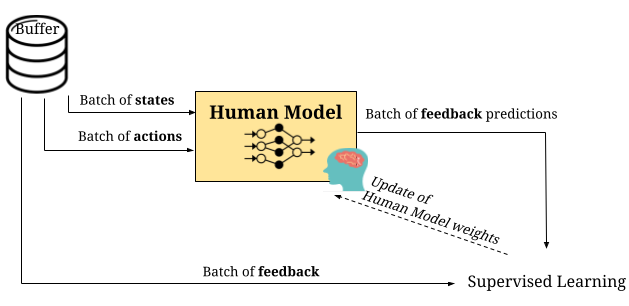
\includegraphics[width=.7\textwidth]{Figures/train_human_model.png}
    \caption{Update of the Human Model}
    \label{fig:update_human_model}
\end{figure}

Figure \ref{fig:update_agent} depicts how the agent's policy will be updated with off-policy corrections indirectly through the Human Model. The Human Model will be able to provide feedback to the newest version of the agent’s policy from a batch of states sampled from the replay buffer. This batch of states will be pass to both the agent's policy and the human model. Then, the agent's policy will output a batch of actions that will be fed to the human model. This batch of actions together with the output of the Human Model will serve to update the weights of the agent's policy. Both models, the agent and the human ones could be learned in parallel.




\begin{figure}[H]
    \centering
    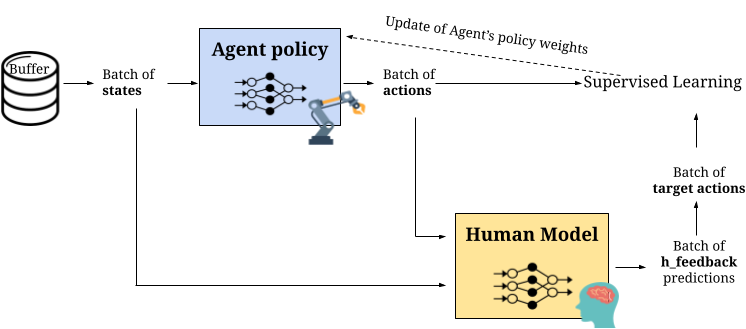
\includegraphics[width=.8\textwidth]{Figures/train_agent.png}
    \caption{Update of the agent's policy}
    \label{fig:update_agent}
\end{figure}




    

